\section{Results}
This chapter will focus on providing key findings derived from the experiment.
The emphasis will be on a comprehensive description of these findings, supported by visual representations. These visualisations serve
as a tool to enhance the clarity of identified trends. The results will be used to evaluate the hypothesis in the discussion section of this report.

\subsection{Relationship between training iterations and loss}
\begin{figure}[h]
   \centering
   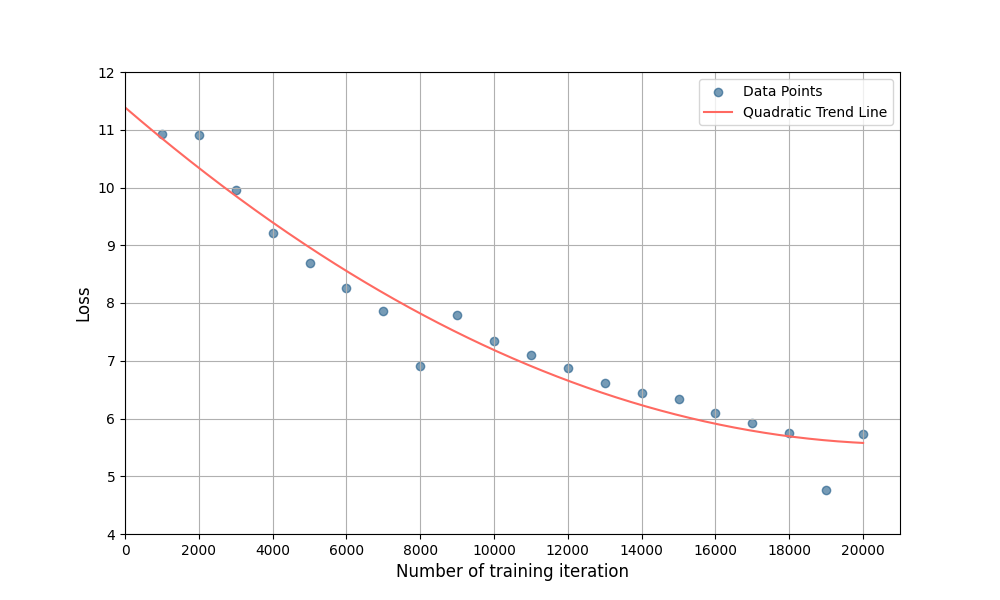
\includegraphics[width=0.9\textwidth]{../Data/loss_by_iteration_plot.png}
   \caption{Quadratic Trend Analysis of Loss Reduction Over 20,000 Training Iterations}
   \label{fig:loss-vs-training-iterations}
\end{figure}
The data illustrated in Fig.\ref{fig:loss-vs-training-iterations} displays the relationship between the the loss of the object detection model over the 20,000 training iterations of the machine learning algorithms. It can be seen that during the initial stages of the experiment, a sharp decline in the loss can be viewed. This demonstrates the initial learning phase of the program. However, with an increased number of training iterations, the rate of the loss decreasing steadily slows down as it approaches its optimal state. \\

The quadratic trendline graphed in Fig.\ref{fig:loss-vs-training-iterations}  displays the model approaching a state of convergence, as the training iteration count increases and loss decreases. Furthermore, the trendline expresses the non-linear relationship between training iterations and the loss of the model. \\
\newpage

\subsection{Relationship between training iterations and accuracy}
The accuracy per class analysis illustrates the model's learning dynamics across different classes.
Figure \ref{fig:accuracy-vs-training-iterations} displays the accuracy per class over 20,000 measured training iterations.
It can be seen that all classes, besides "Person", rapidly increase after around 2000 training iterations. After 10,000 iterations
all of these classes have an accuracy of roughly 80\%. Over the next 10,000 iterations, the accuracy then slowly approaches 95 to 100\%.
This is different for "Person", which after 1000 iterations already starts with an accuracy of about 35\% and a steep incline to 97\%
after 5500 iterations. After that it slowly approaches 100\% accuracy.
Important to note is the fluctuation of accuracy for "Dog" and "Wheel" at 13,000 and 14,000 iterations respectively.

\begin{figure}[h]
   \centering
   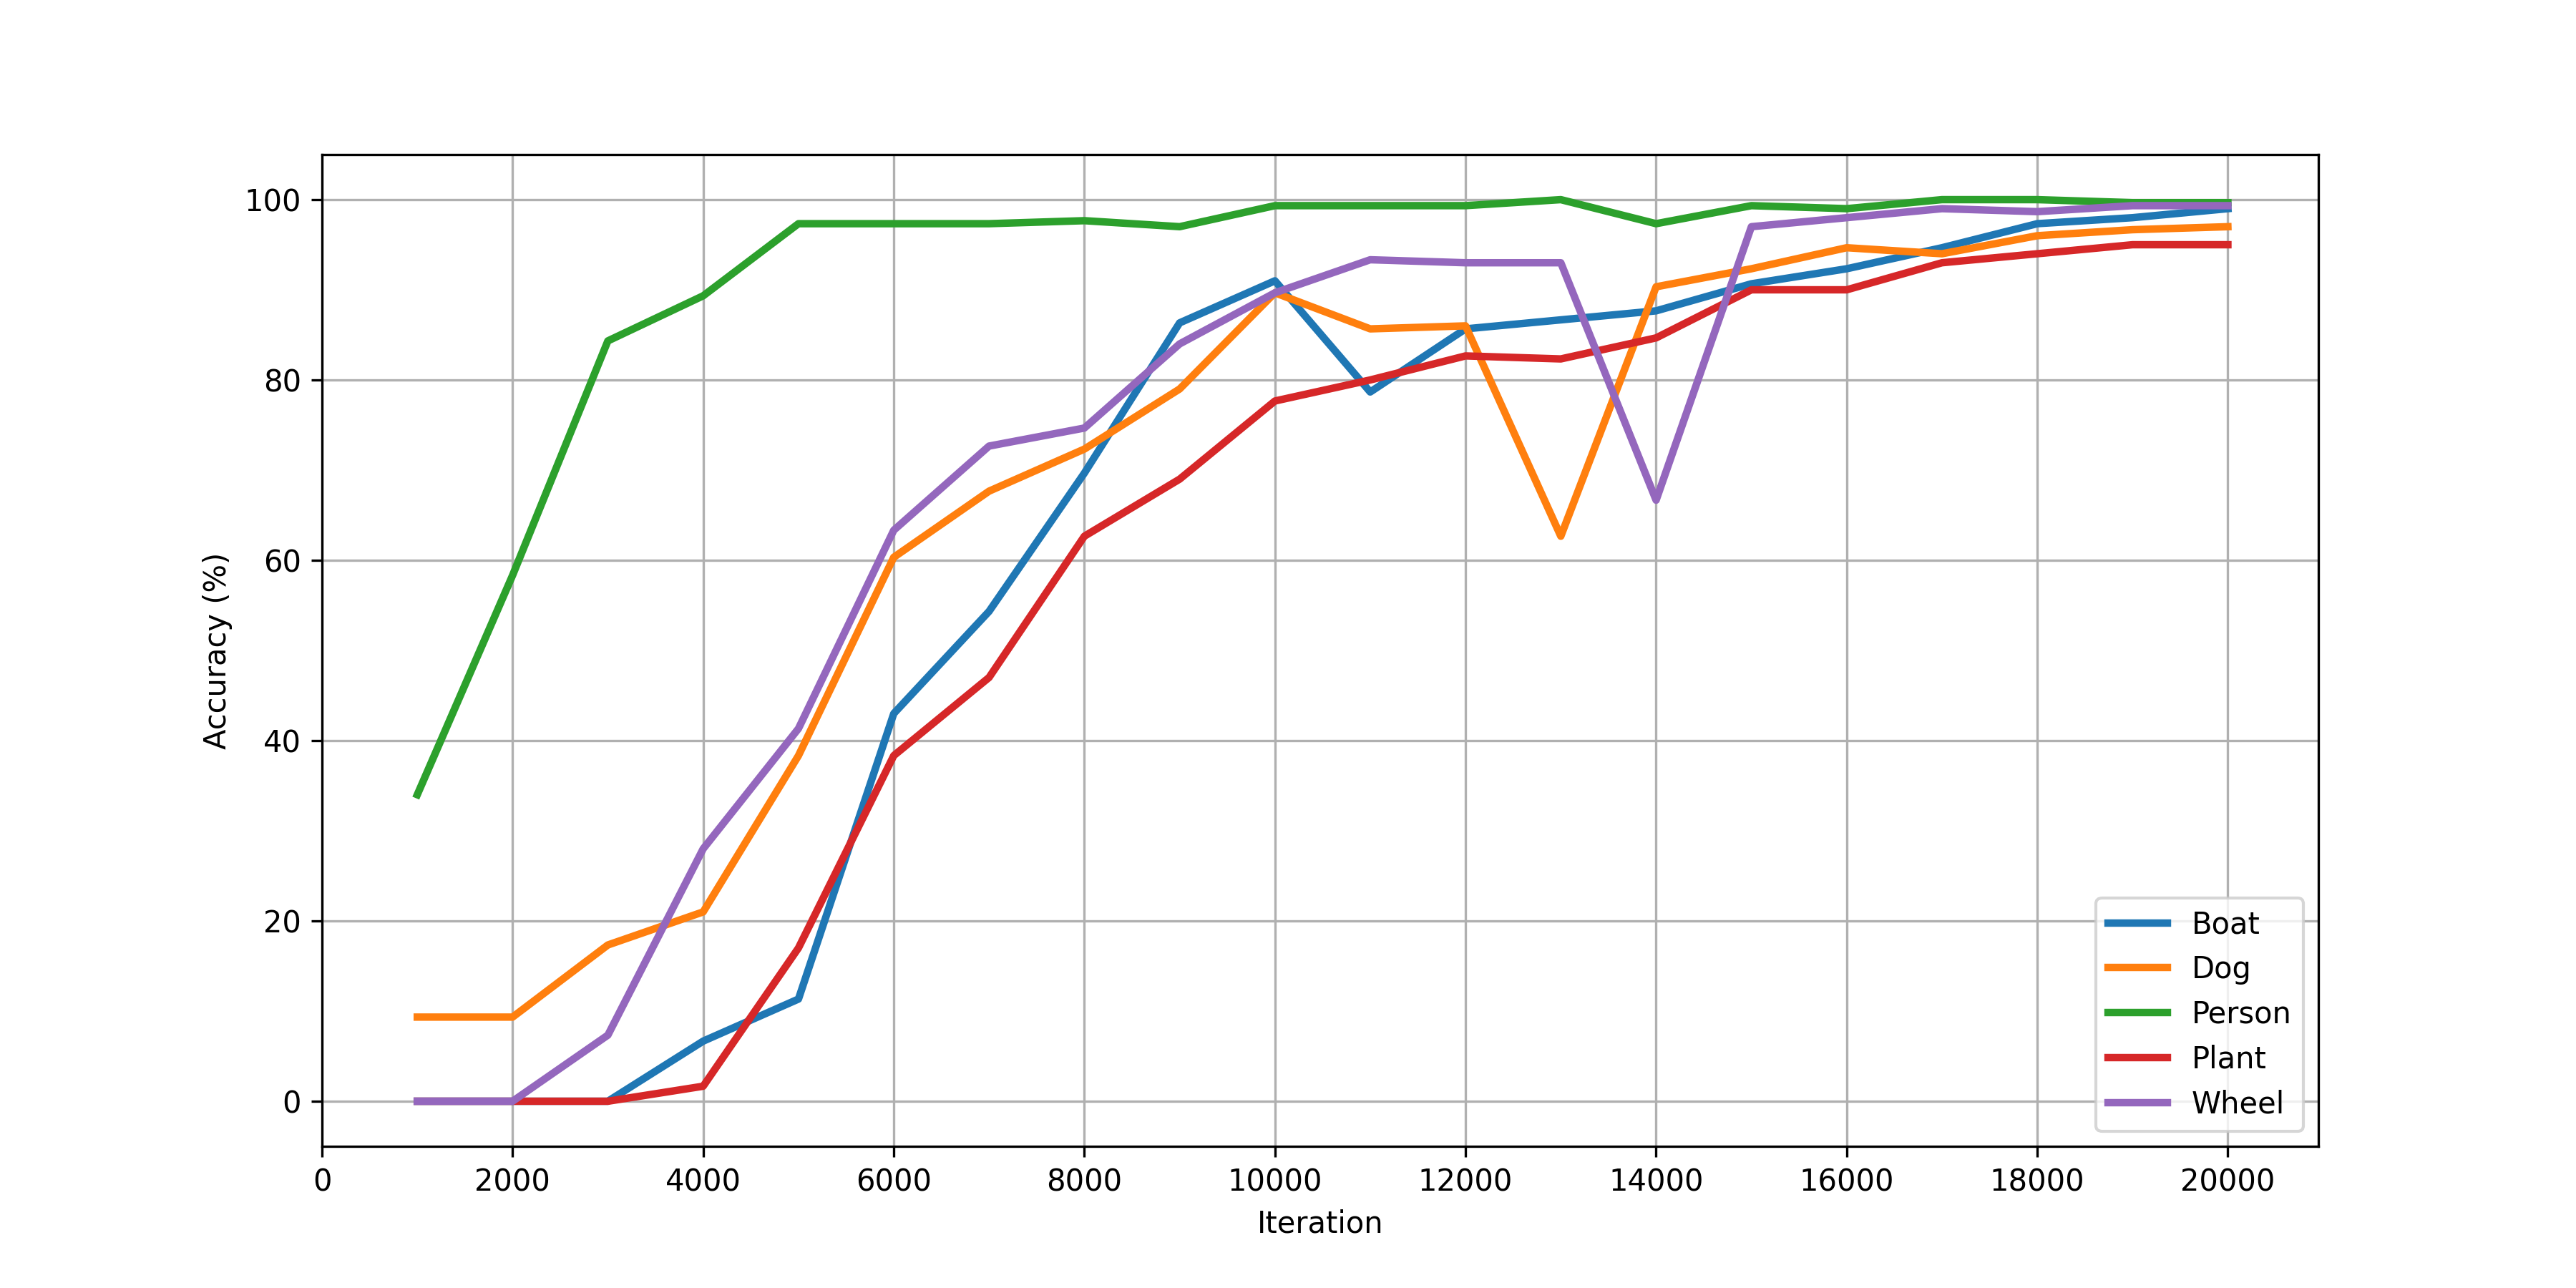
\includegraphics[width=0.9\textwidth]{../Data/accuracy-graph.png}
   \caption{Accuracy per Class over 20,000 Training Iterations}
   \label{fig:accuracy-vs-training-iterations}
\end{figure}


To assess the overall performance of the model, the average accuracy per iteration and its rate of change were calculated.
The "Average Accuracy" in Figure \ref{fig:accuracy-improvement} displays the aggregated information seen in Figure 
\ref{fig:accuracy-vs-training-iterations}. The aggregation of data attenuates the fluctuation seen for the classes "Dog" and "Wheel" 
(See Fig. \ref{fig:accuracy-vs-training-iterations}) and thus making the the upward trend between 10,000 and 20,000 iterations more visible.
\\
The model starts off with a substantial increase in accuracy, which is followed by a dip in the rate of change, as the rise in accuracy 
decelerates. A further steep incline can be detected between 4000 and 6000 iterations, which is followed by a steady increase in accuracy, as
the rate of change falls. A small dip in accuracy can be seen at iteration 11,000, after which a bigger anomaly occurs between 13,000
and 14,000 iterations. Following the dip, the model resumes its positive uptrend trend, reaching an average performance of 98\% after its final
iteration (20,000).
\newpage

\begin{figure}[h]
   \centering
   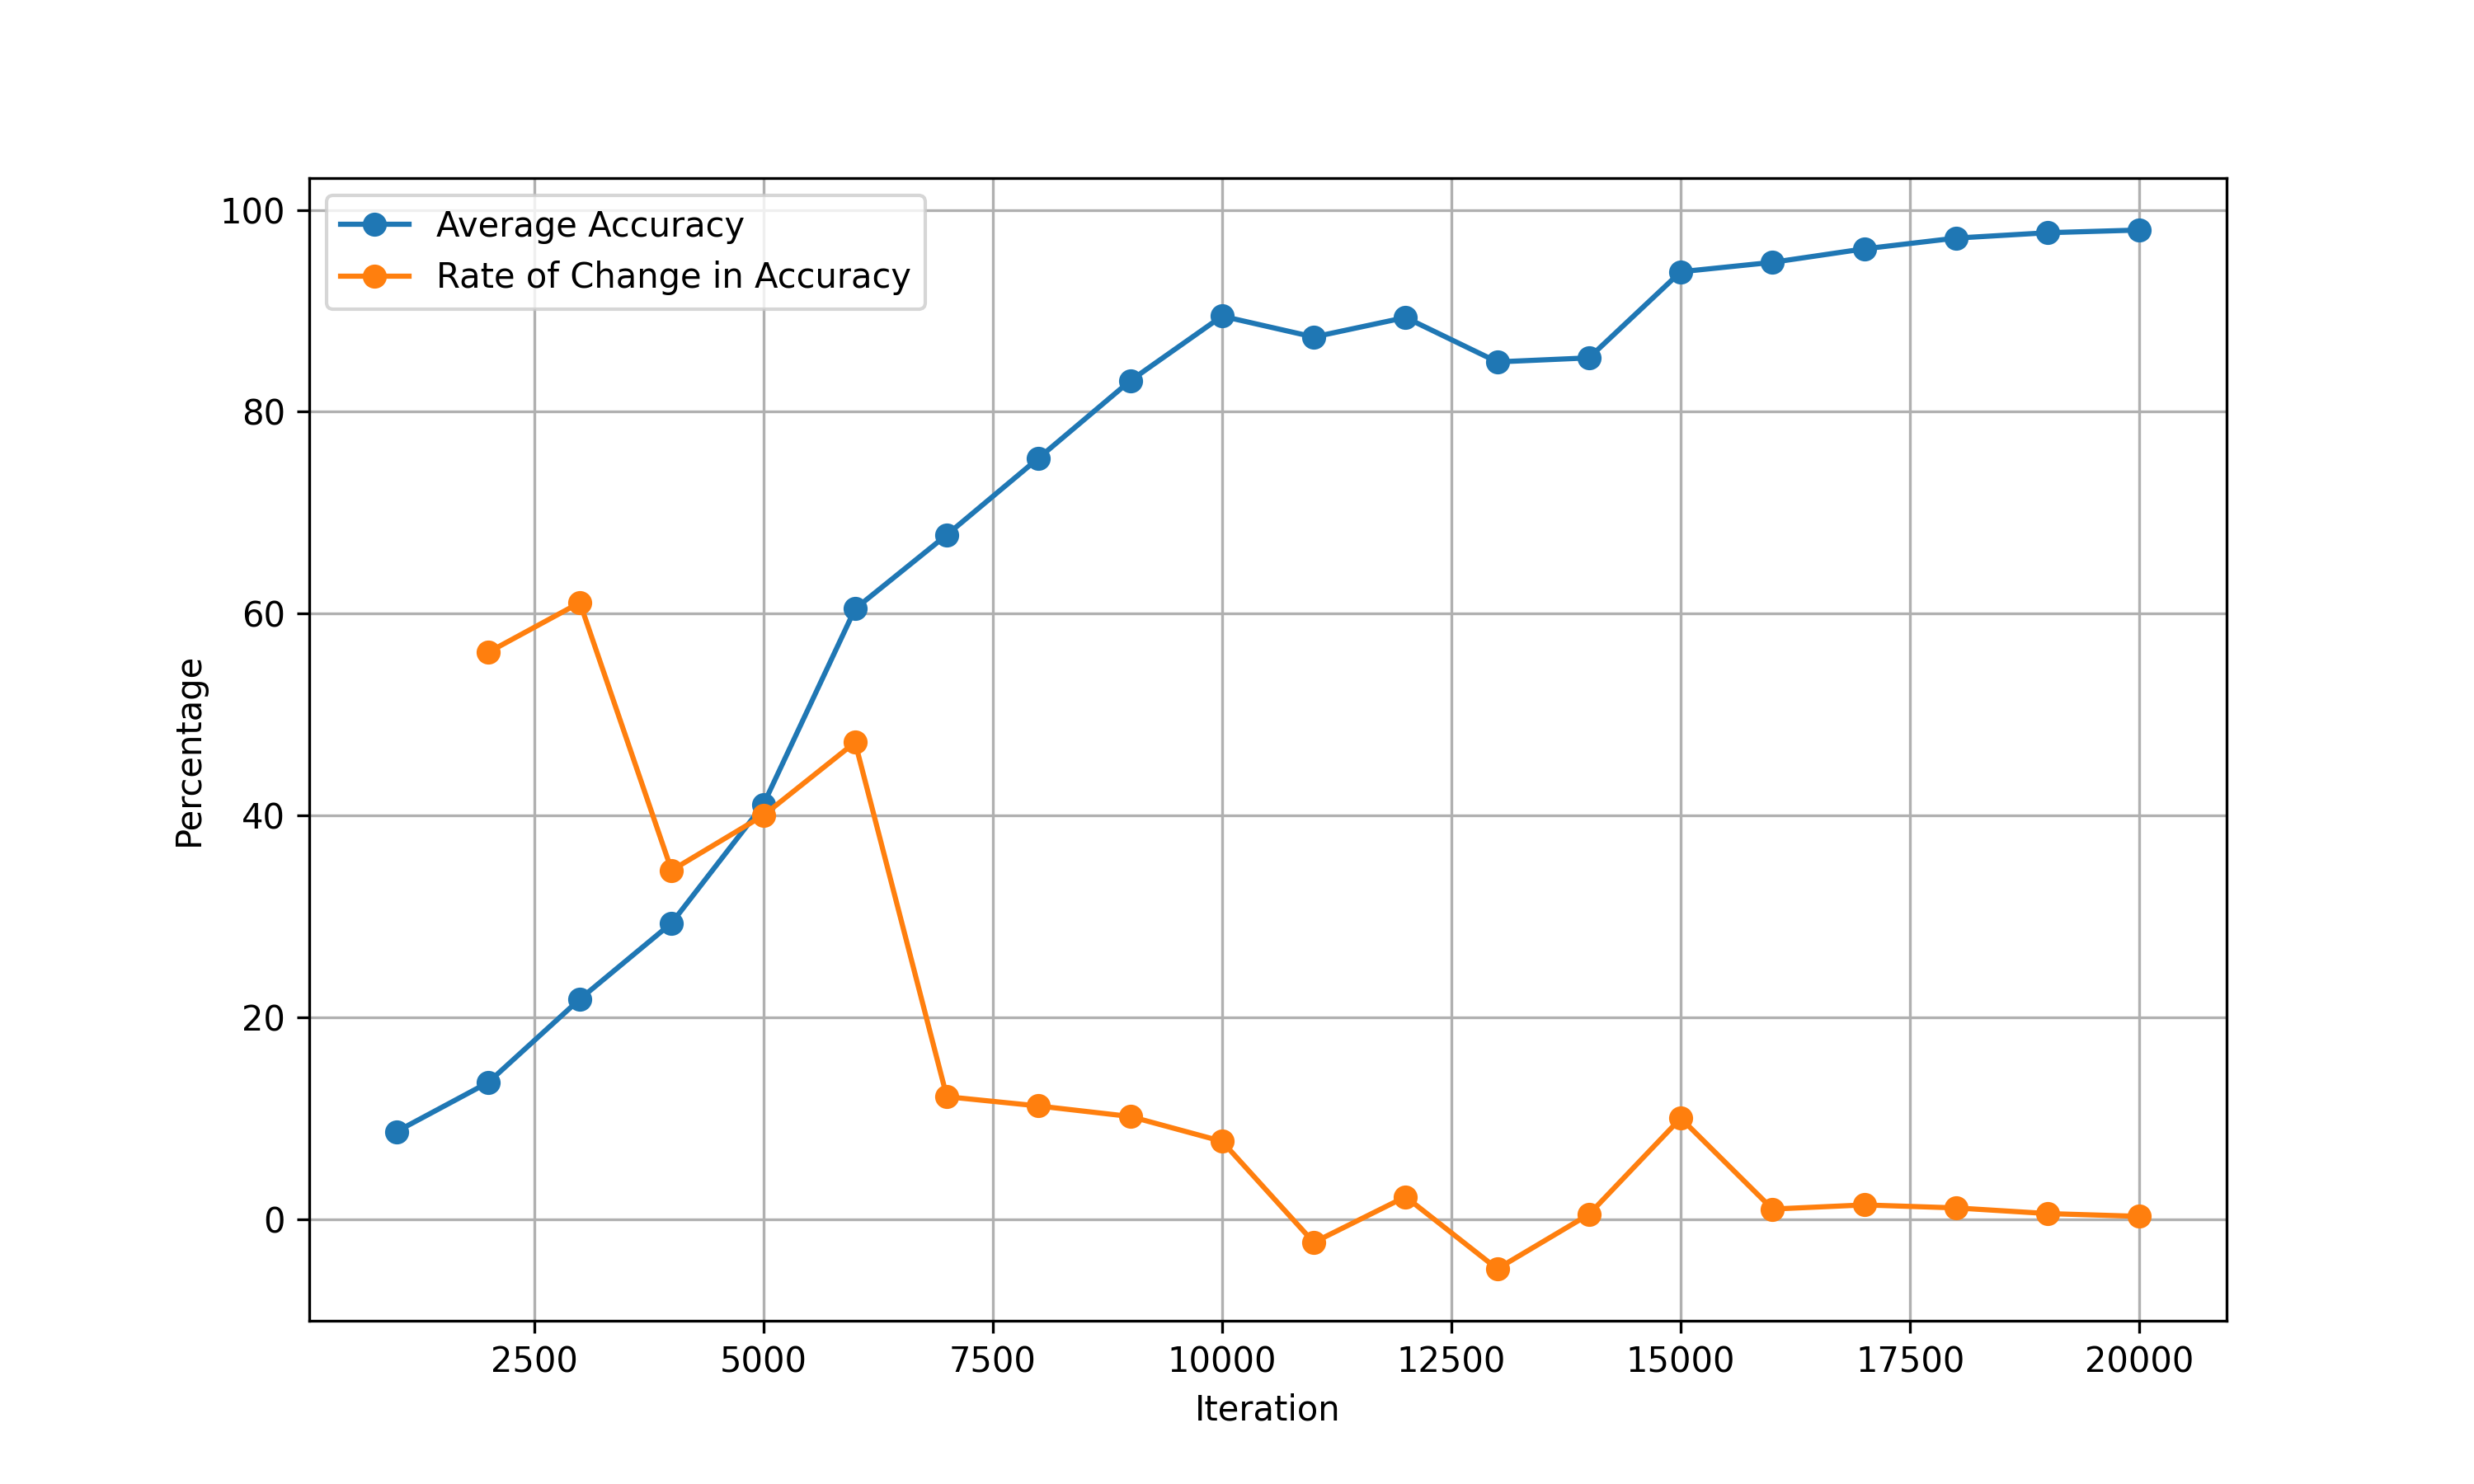
\includegraphics[width=0.9\textwidth]{../Data/accuracy-improvement-graph.png}
   \caption{Average Accuracy and its Rate of Change}
   \label{fig:accuracy-improvement}
\end{figure}

Overall, the chart depicts a generally positive trajectory for the average accuracy, with a few outliers. The "Rate of Change" emphasizes
key points in the model's learning process and makes instances in which the average accuracy experiences notable increases or decreases more
visible. The described fluctuation in accuracy needed to be further investigated, hinting at possible
challenges in the learning process of the object detection model. \\

\subsection{Analysing fluctuation in loss and accuracy}

The data reveals a notable decline in accuracy at 13,000 training iterations for the dog class and 14,000 training iterations for the wheel class, respectively. To further investigate the observed downturns in the data, analysing the average data points displaying the decline can provide a more comprehensive insight. The data points displayed in Figure (----) for each class represent the average accuracy score of three images. 
\newpage
\begin{figure}[h]
   \centering
   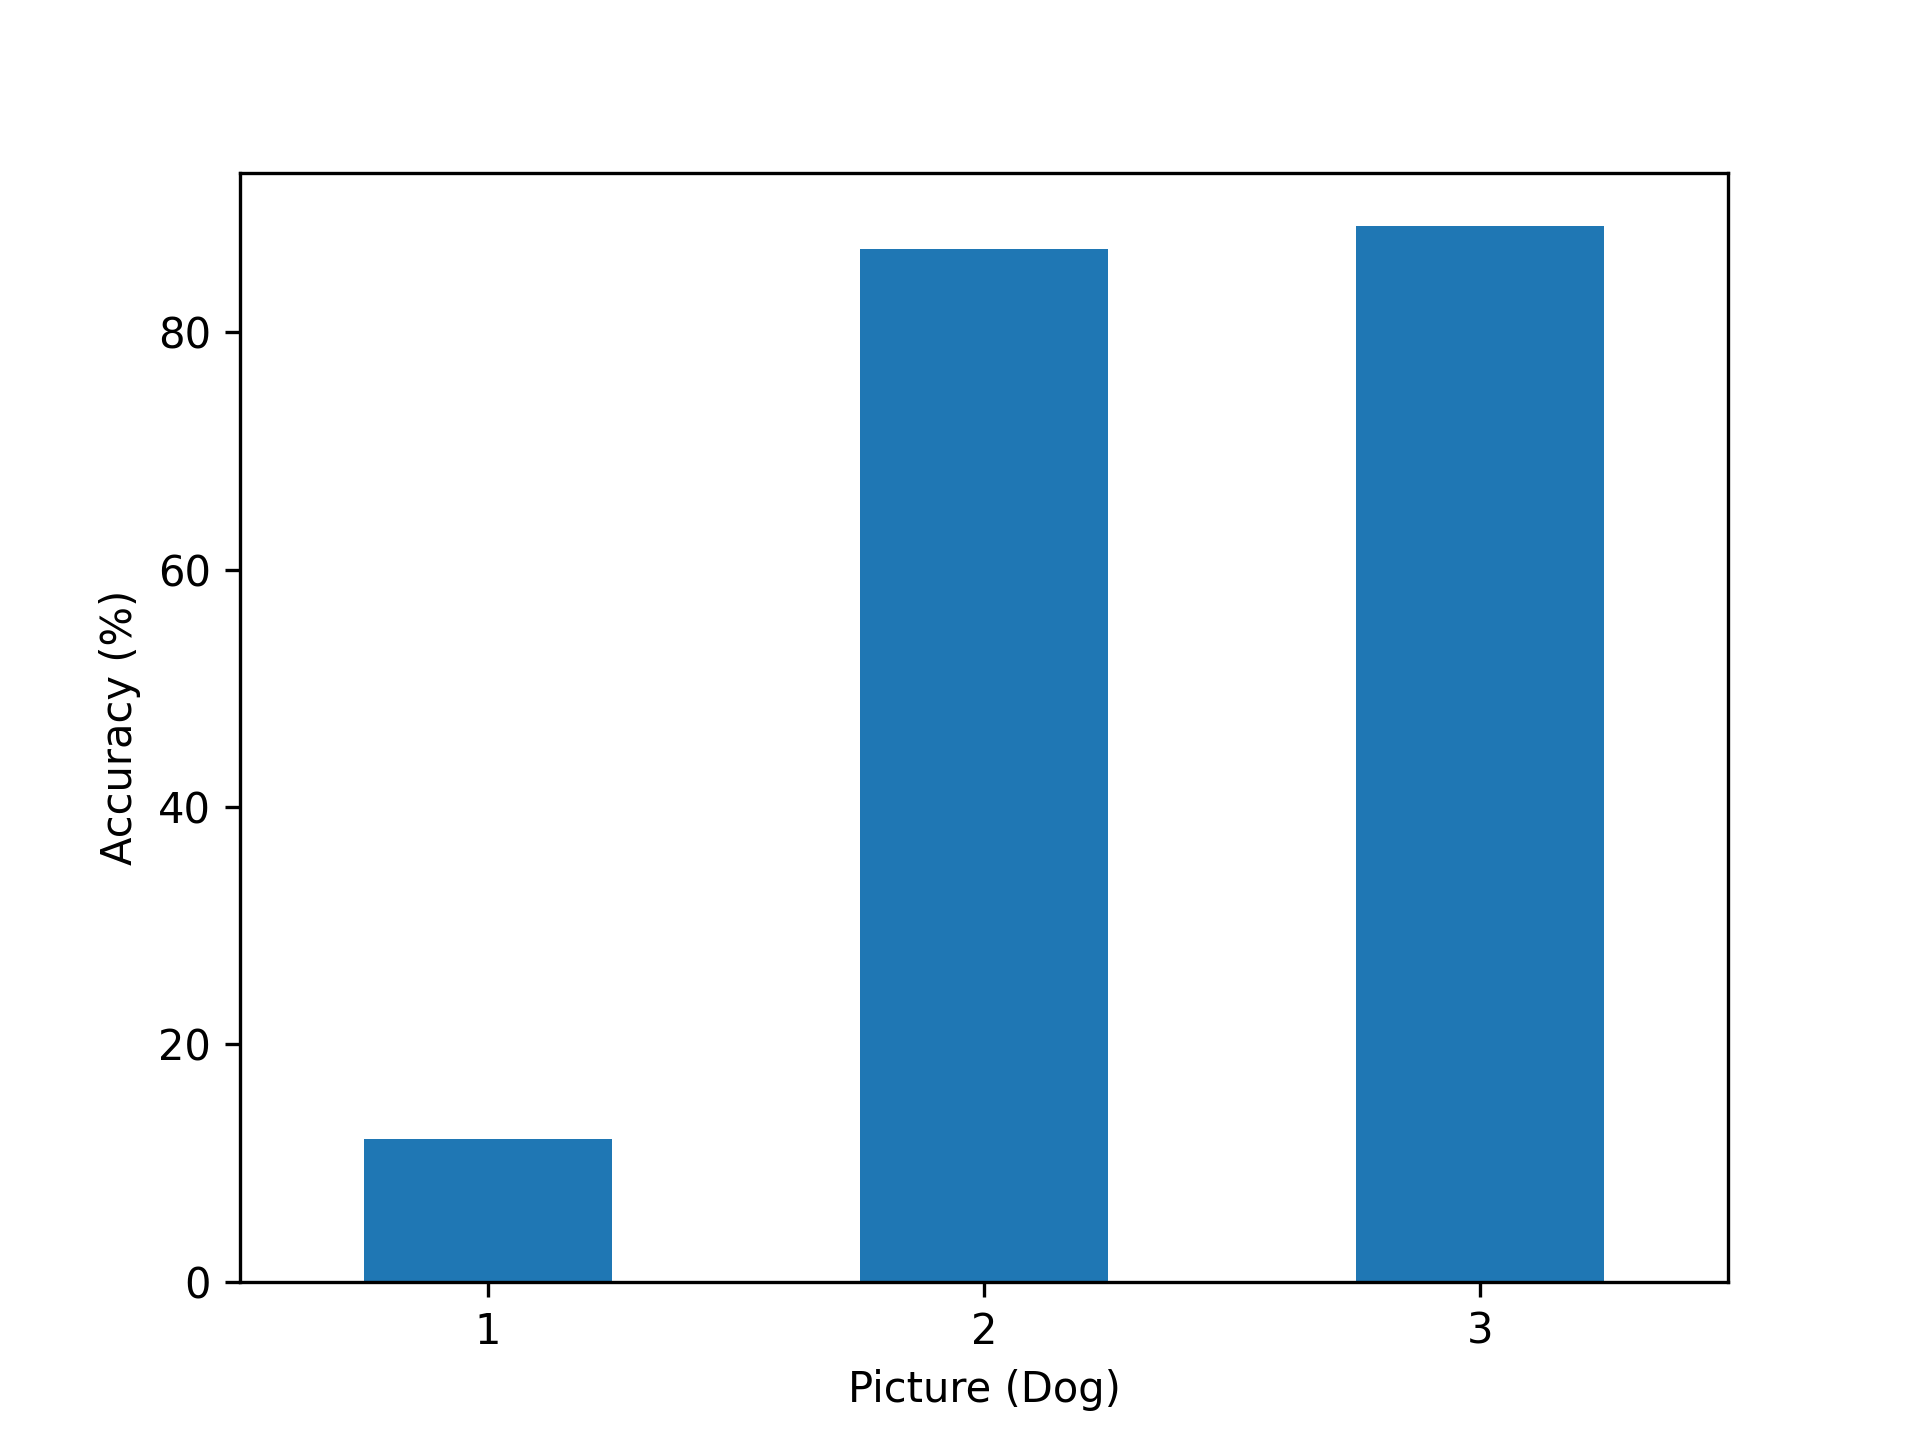
\includegraphics[width=0.5\textwidth]{../Data/dog-outliers.png}
   \caption{Accuracy Discrepancy Among Images in Dog Class at 13,000 Training Iterations}
   \label{fig:14000-dog}
\end{figure}

Figure \ref{fig:14000-dog} displays three different instances of the dog class that make up the average data point for 13,000 training iterations, at which the dip in data was observed. The graph in Figure \ref{fig:14000-dog} reveals the accuracy score obtained by each image during this iteration test. Notable both images 2 and 3 receive high accuracy scores with 87 and 89 percentage points respectively. On the other hand image 1 only has an accuracy of 12 percentage points, showing an anomaly in the data.

\begin{figure}[h]
   \centering
   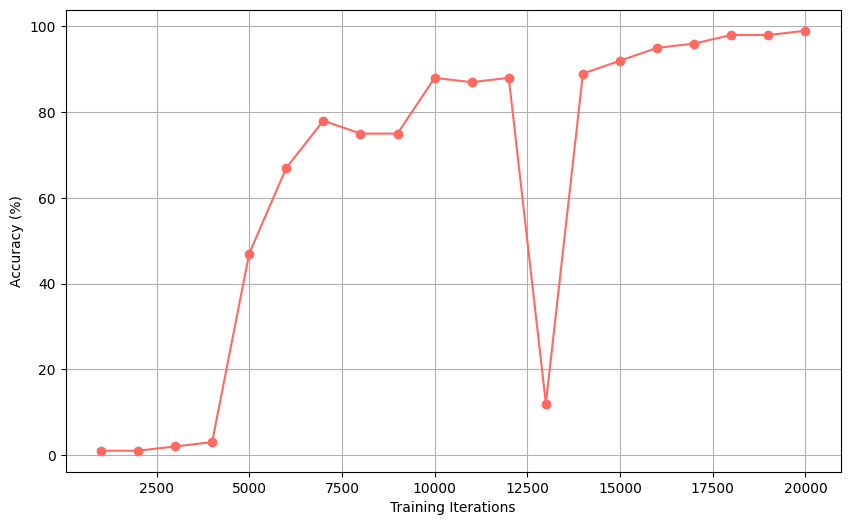
\includegraphics[width=0.5\textwidth]{../Data/dogs_image1_accuracy_vs_iteration.png}
   \caption{Dog Class Image 3 Training Iterations vs. Accuracy }
   \label{fig:image-1-accuracy}
\end{figure}

To further illustrate and investigate the dip in accuracy in the dog class, and the found anomaly in image 1,  Figure \ref{fig:image-1-accuracy} can be utilised, which displays the relationship between accuracy and training interaction for image 1. Notable in this Figure, is that the previously discovered anomaly of 12 percent at 13,000 training iterations is also clearly represented in the graph at the steep dip. This data point is a significant deviation from the otherwise existing pattern, displaying a clear divergence from the expected accuracy trajectory. Therefore it can be concluded that this data point represents an outlier in the data. Reasons for such an outlier will be evaluated in the discussion chapter. 
\newpage

\begin{figure}[h]
   \centering
   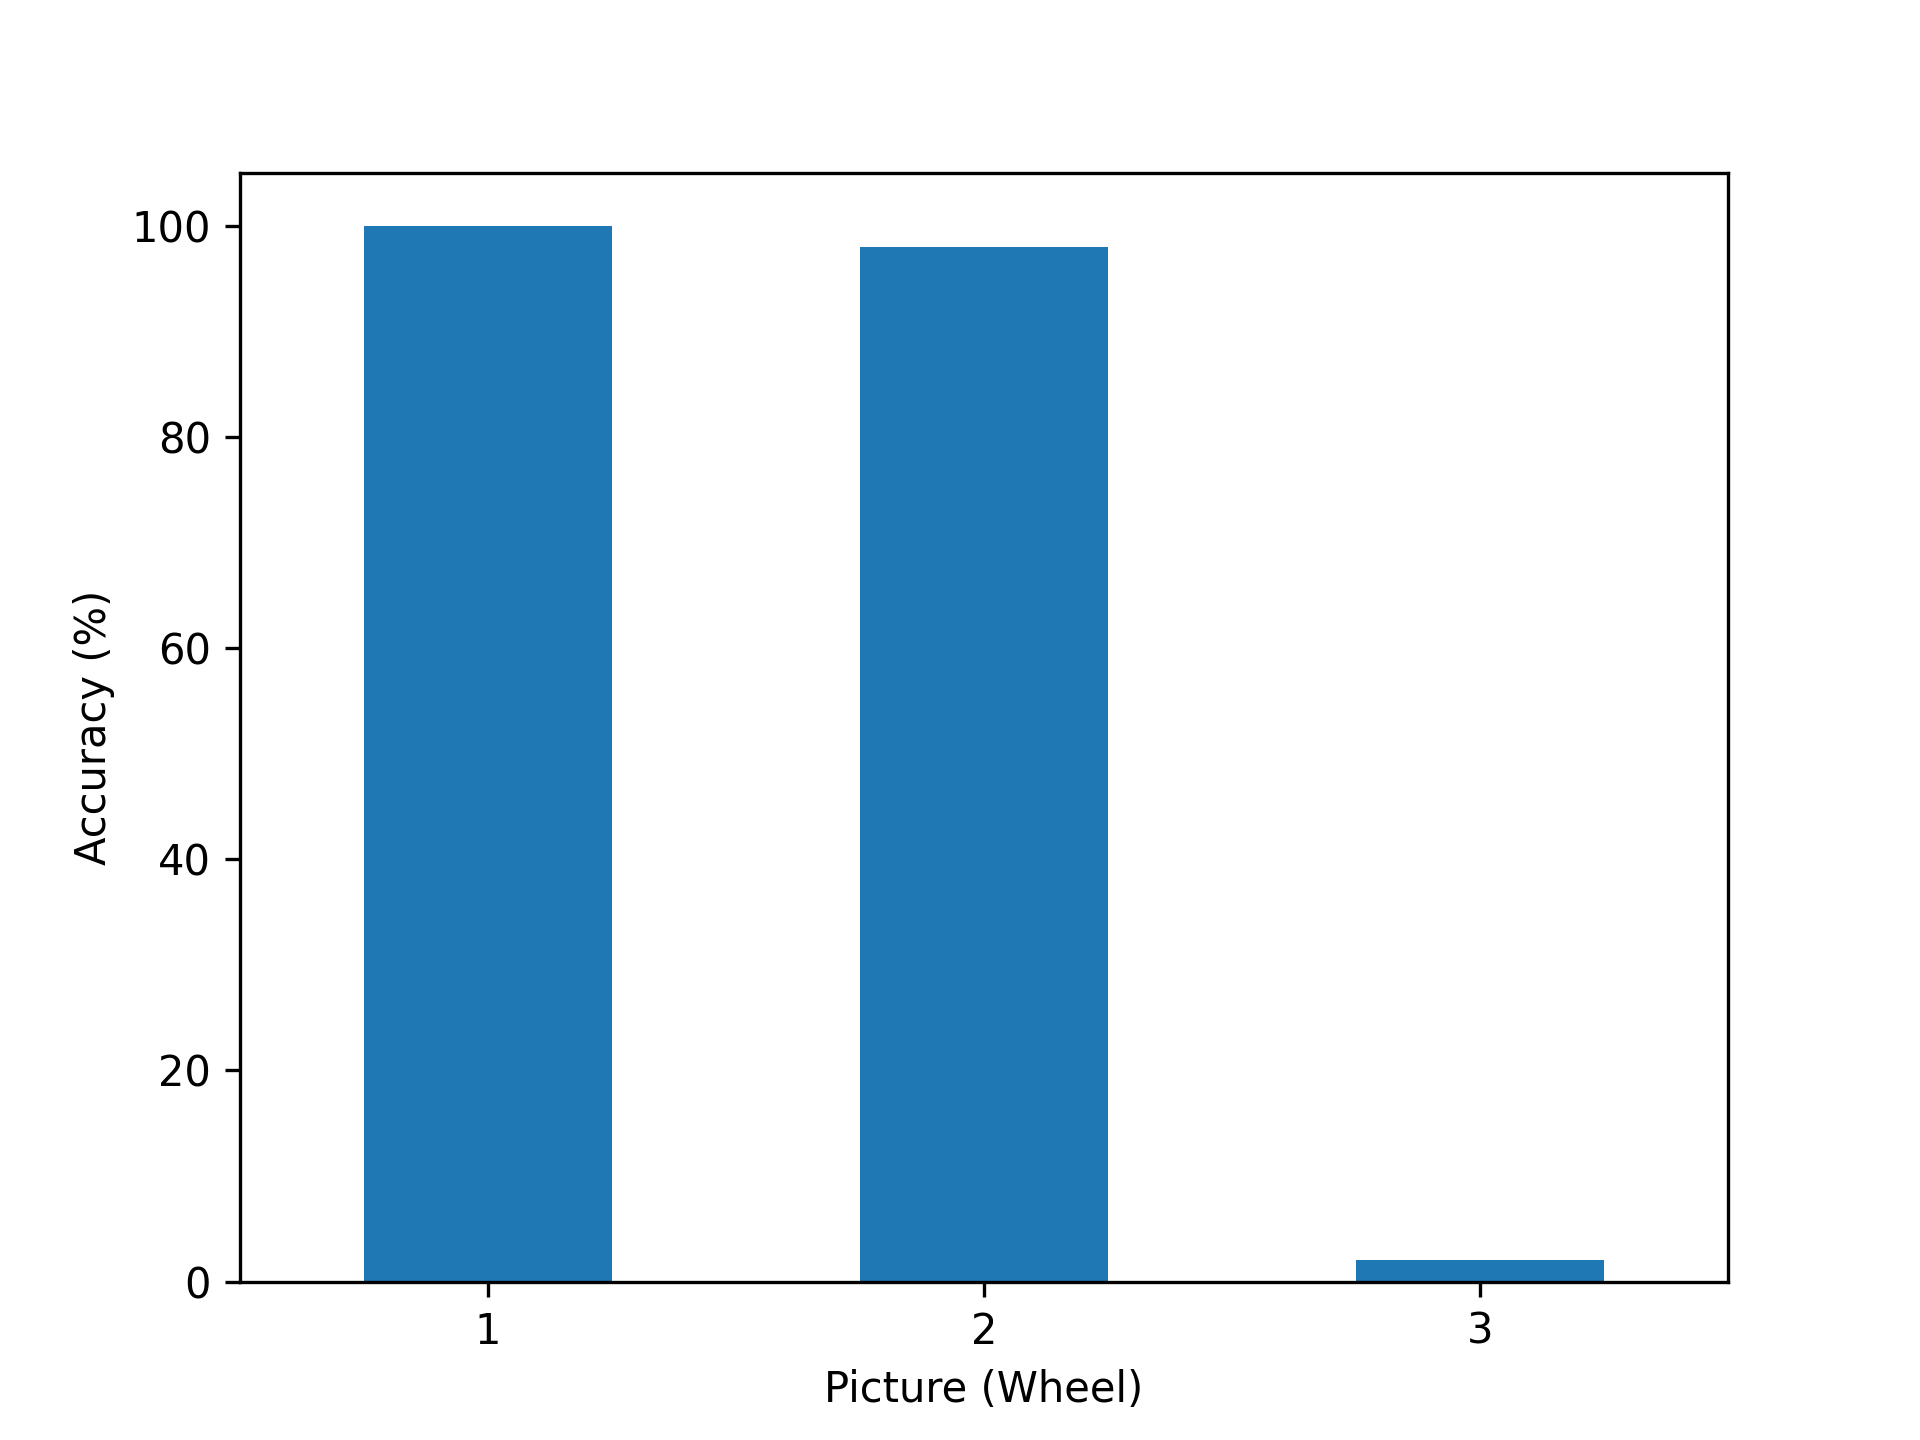
\includegraphics[width=0.5\textwidth]{../Data/wheel-outliers.png}
   \caption{Accuracy Discrepancy Among Images in Whell Class at 14,000 Training Iterations}
   \label{fig:13000-wheel}
\end{figure}

A similar analysis can be drawn for the wheel class, in Figure \ref{fig:13000-wheel} the accuracy score for the three instances of the wheel class at 14,000 training iterations can be observed. Whilst images 1 and 2 received 100 percent and 98 percent accuracy, image 3 displays as a clear anomaly with only 2 percent accuracy. 


\begin{figure}[h]
   \centering
   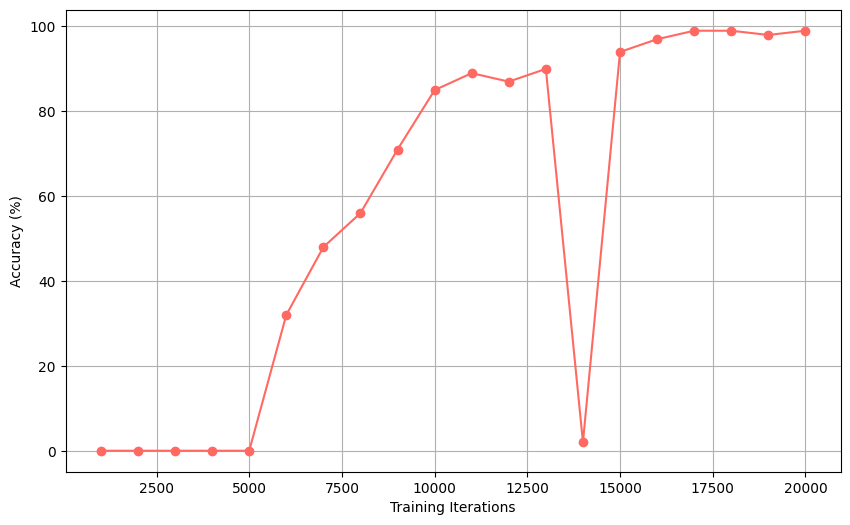
\includegraphics[width=0.5\textwidth]{../Data/wheel_image1_accuracy_vs_iteration.png}
   \caption{Dog Class Image 3 Training Iterations vs. Accuracy }
   \label{fig:image-3-accuracy}
\end{figure}

To further analyse the cause of the anomaly found at 14,000 iterations in image 3, figure \ref{fig:image-3-accuracy} can be utilised, displaying the accuracy of image 3 in the wheel class over 20,000 iterations. This graph illustrates that the given anomaly does not follow the data trend, but rather deviates from the accuracy trajectory, due to its considerably lower accuracy score. Consequently, this data point can also be classified as an outlier, this will be further examined in the discussion chapter. \\
\newpage


\subsection{Distribution of model accuracy across training iterations}

\begin{figure}[h]
   \centering
   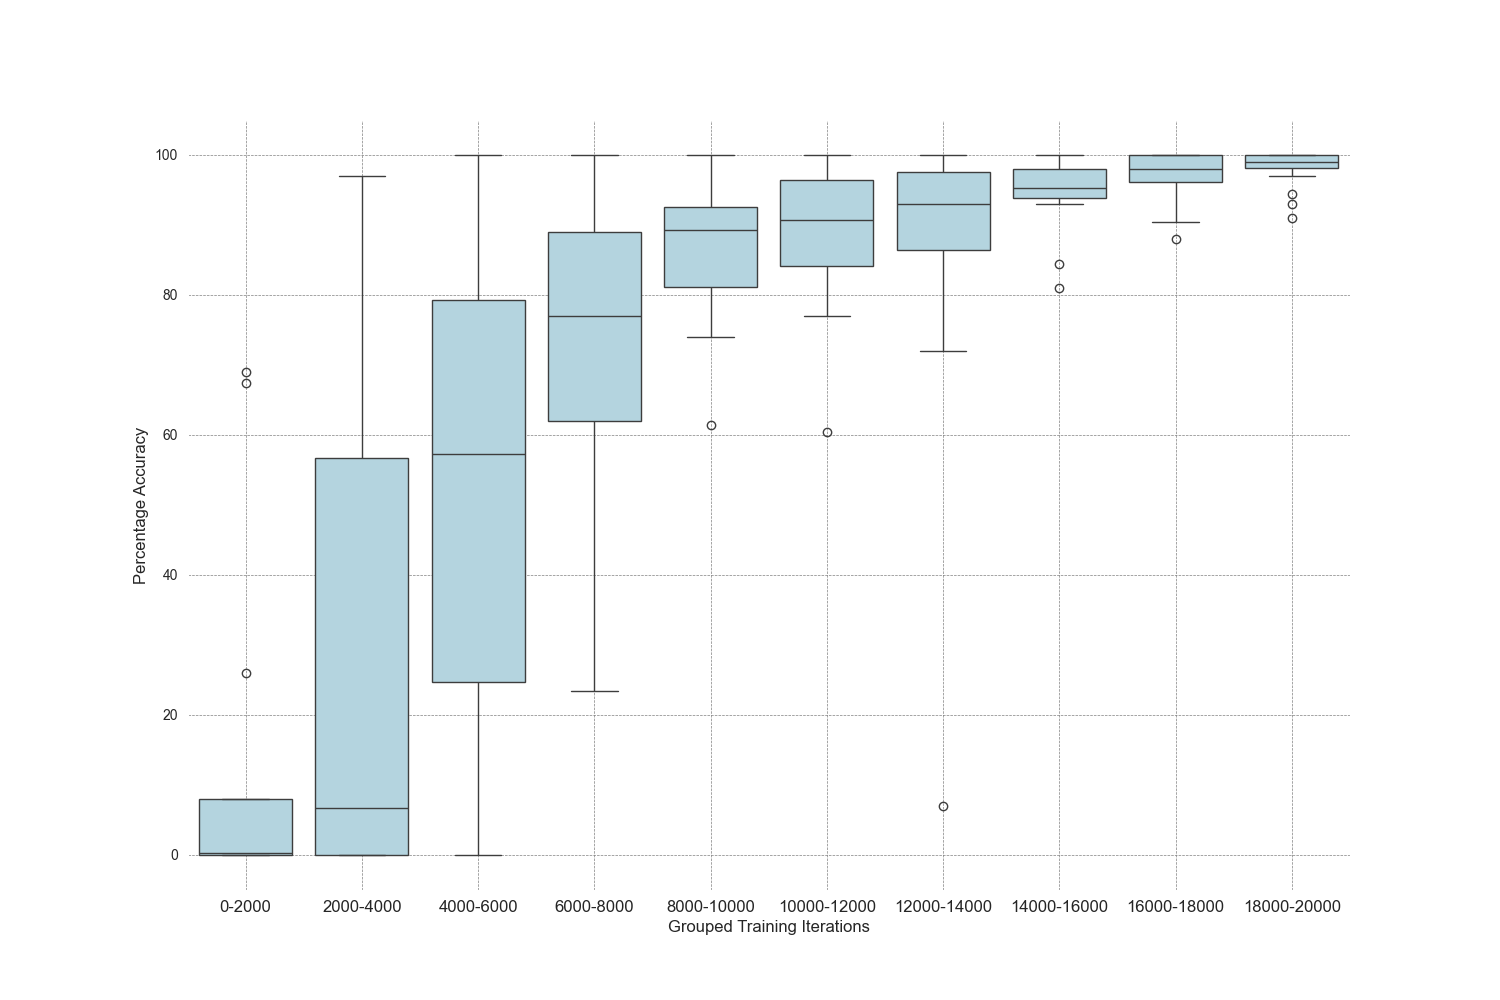
\includegraphics[width=0.9\textwidth]{../Data/box_plot_iteration_vs_accuracy.png}
   \caption{Box Plot of Model Accuracy Across Different Training Iteration Groups}
   \label{fig:Box-plot}
\end{figure}


The following Figure \ref{fig:Box-plot} illustrates a comprehensive overview of the changes in the model's accuracy throughout 20,000 training iterations. It displays the distribution and tendencies of the accuracy throughout the training process in relation to the entire model.\\

Initially, the Figure displays an initial surge in model accuracy up to 4000 iterations. From this point onwards, the median accuracy stabilizes and the variance diminishes in the 4000-12000 training iteration range. Beyond 12000 iterations, there is only minimal change in the median accuracy, signalling the onset of a plateau. Thereafter the graph displays that with further training, only a slight decrease in variance and an increase in median is achieved. \\

One key aspect that the box plot highlights is the changes in data variability throughout the model's training process. Initially, a greater degree of variability is displayed, especially in the grouped 2000-4000 training iteration block. Here the interquartile range (IQR) is notably wider, clearly displaying the greater spread of different accuracy scores.  However, as the training iteration count increases, the range of the spread decreases. The IQR becomes progressively narrower in the higher training iteration groups, indicating a decrease in variability. \\









